\documentclass[border=10pt]{standalone}
\usepackage{tikz}
\usetikzlibrary{shapes.geometric, arrows, positioning, fit}

% Define block styles
\tikzstyle{startstop} = [rectangle, rounded corners, minimum width=3cm, minimum height=1cm, text centered, draw=black, fill=red!30]
\tikzstyle{process} = [rectangle, minimum width=3cm, minimum height=1cm, text centered, draw=black, fill=blue!30]
\tikzstyle{decision} = [diamond, minimum width=3cm, minimum height=1cm, text centered, draw=black, fill=green!30]
\tikzstyle{arrow} = [thick,->,>=stealth]

\begin{document}
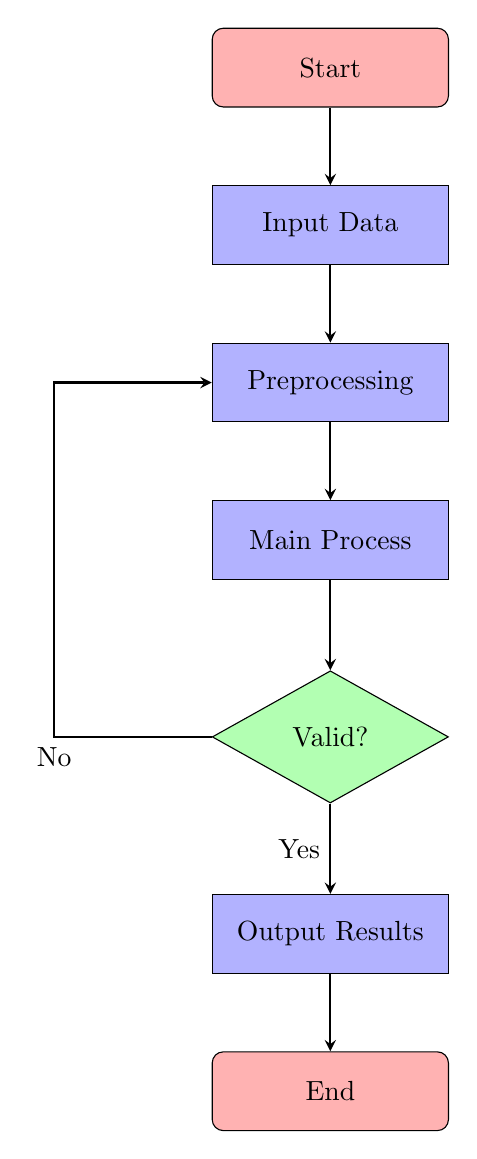
\begin{tikzpicture}[node distance=2cm]

% Nodes
\node (start) [startstop] {Start};
\node (input) [process, below of=start] {Input Data};
\node (process1) [process, below of=input] {Preprocessing};
\node (process2) [process, below of=process1] {Main Process};
\node (decision) [decision, below of=process2, yshift=-0.5cm] {Valid?};
\node (output) [process, below of=decision, yshift=-0.5cm] {Output Results};
\node (stop) [startstop, below of=output] {End};

% Arrows
\draw [arrow] (start) -- (input);
\draw [arrow] (input) -- (process1);
\draw [arrow] (process1) -- (process2);
\draw [arrow] (process2) -- (decision);
\draw [arrow] (decision) -- node[anchor=east] {Yes} (output);
\draw [arrow] (decision) -| node[anchor=north] {No} ([xshift=-2cm]process1.west) |- (process1);
\draw [arrow] (output) -- (stop);

\end{tikzpicture}
\end{document}

